\section{Climate Change Ontology}\label{sec:result_cc_ontology}
In this section, results from the crowd-sourced ontology validation in the field of climate change are presented. A detailed discussion of the ontology used as a baseline for all calculations was done previously in \hyperref[sec:evaluation_datasets]{Section~\ref*{sec:evaluation_datasets}}. 

The results of the benchmark are presented in~\hyperref[table:bench_p_r_f_climate_change]{Table~\ref*{table:bench_p_r_f_climate_change}}. For comparison, we also performed ontology validation without any of the discussed Context enrichment methods~\emph{(None)}. Given the relatively small number of concepts, all Context enrichment methods performed better than having no Context at all. Surprisingly, in terms of Recall the contrary holds. Indeed, crowd workers tend to negatively answer questions in case of uncertainty or when no additional information other than the concept name is present. 
\begingroup
\renewcommand{\arraystretch}{1.5}
\begin{table}
	\begin{tabularx}{\textwidth}{l c*{3}{Y}}
		\toprule
		Method & Precision & Recall & F-Measure \\
		\midrule
		 Ontology based Approach & 0.758 & 0.805 & 0.781 \\
		 Metadata based Approach & 0.732 & 0.831 & 0.778 \\
		 Dictionary based Approach & 0.724 & 0.821 & 0.769 \\
		 None & 0.549 & 0.837 & 0.663 \\
		\bottomrule
	\end{tabularx}
	\caption{Aggregated results on the Climate Change Ontology~(ranked by F-Measure)}
	\label{table:bench_p_r_f_climate_change}
\end{table}
\endgroup

We also measured the agreement ratio~(Inter-rater Agreement) in this dataset. \hyperref[fig:hist_agreement_climate_change_all]{Figure~\ref*{fig:hist_agreement_climate_change_all}} shows the distribution of the agreement ratio among all validated concepts. We required 5 judgements for every concept, yielding $5/0$, $4/1$ or $3/2$ levels of agreement, which is equivalent to
\emph{full agreement}~($1.0$), \emph{partial agreement}~($0.8$) and \emph{little agreement}~($0.6$) respectively. 
\begin{sidewaysfigure}
  	 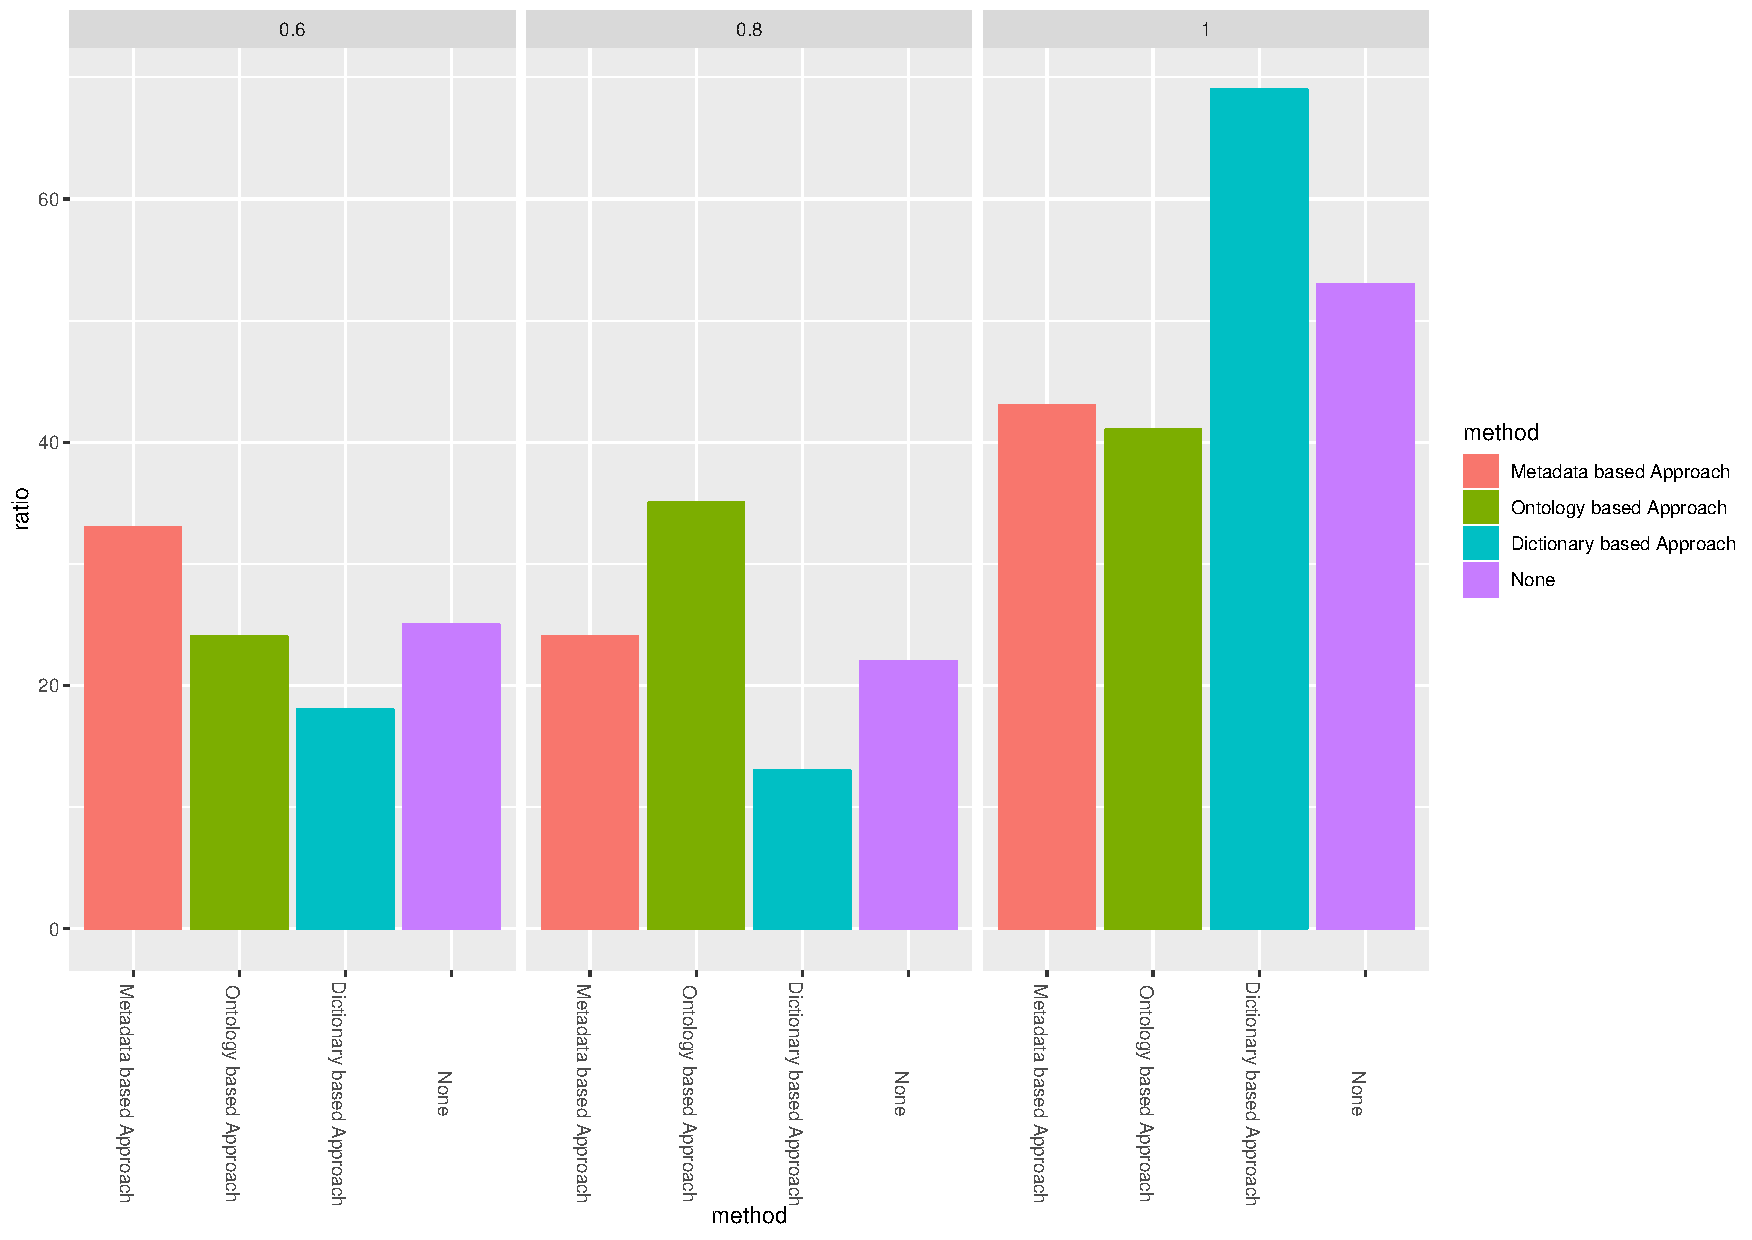
\includegraphics[width=\textwidth]{plots/climate_change/hist_agreement_corrected}
  	 \caption{Histogram plots of the Inter-rater Agreement}\label{fig:hist_agreement_climate_change_all}
\end{sidewaysfigure}

The highest agreement exhibits the \emph{Dictionary~based~Approach}, followed by \emph{None}. This is somewhat interesting as these are the methods with the lowest performance with regard to F-Measure. In fact, the agreement ratio just describes to what extent the responses coincide. From the observations in this dataset, it is hard, if not impossible, to draw conclusions solely based on agreement. In fact, when looking closely at the judgements with the highest agreement~ratio among incorrect answers, $16$ of $17$ judgements for the Dictionary~based~Approach and $3$ of $6$ judgements for the Ontology~based~Approach had Context added. Apparently, crowd workers agreed here on incorrect values even though concept descriptions were available. 

\begin{figure}
    \centering
    \begin{subfigure}[b]{0.4\textwidth}
        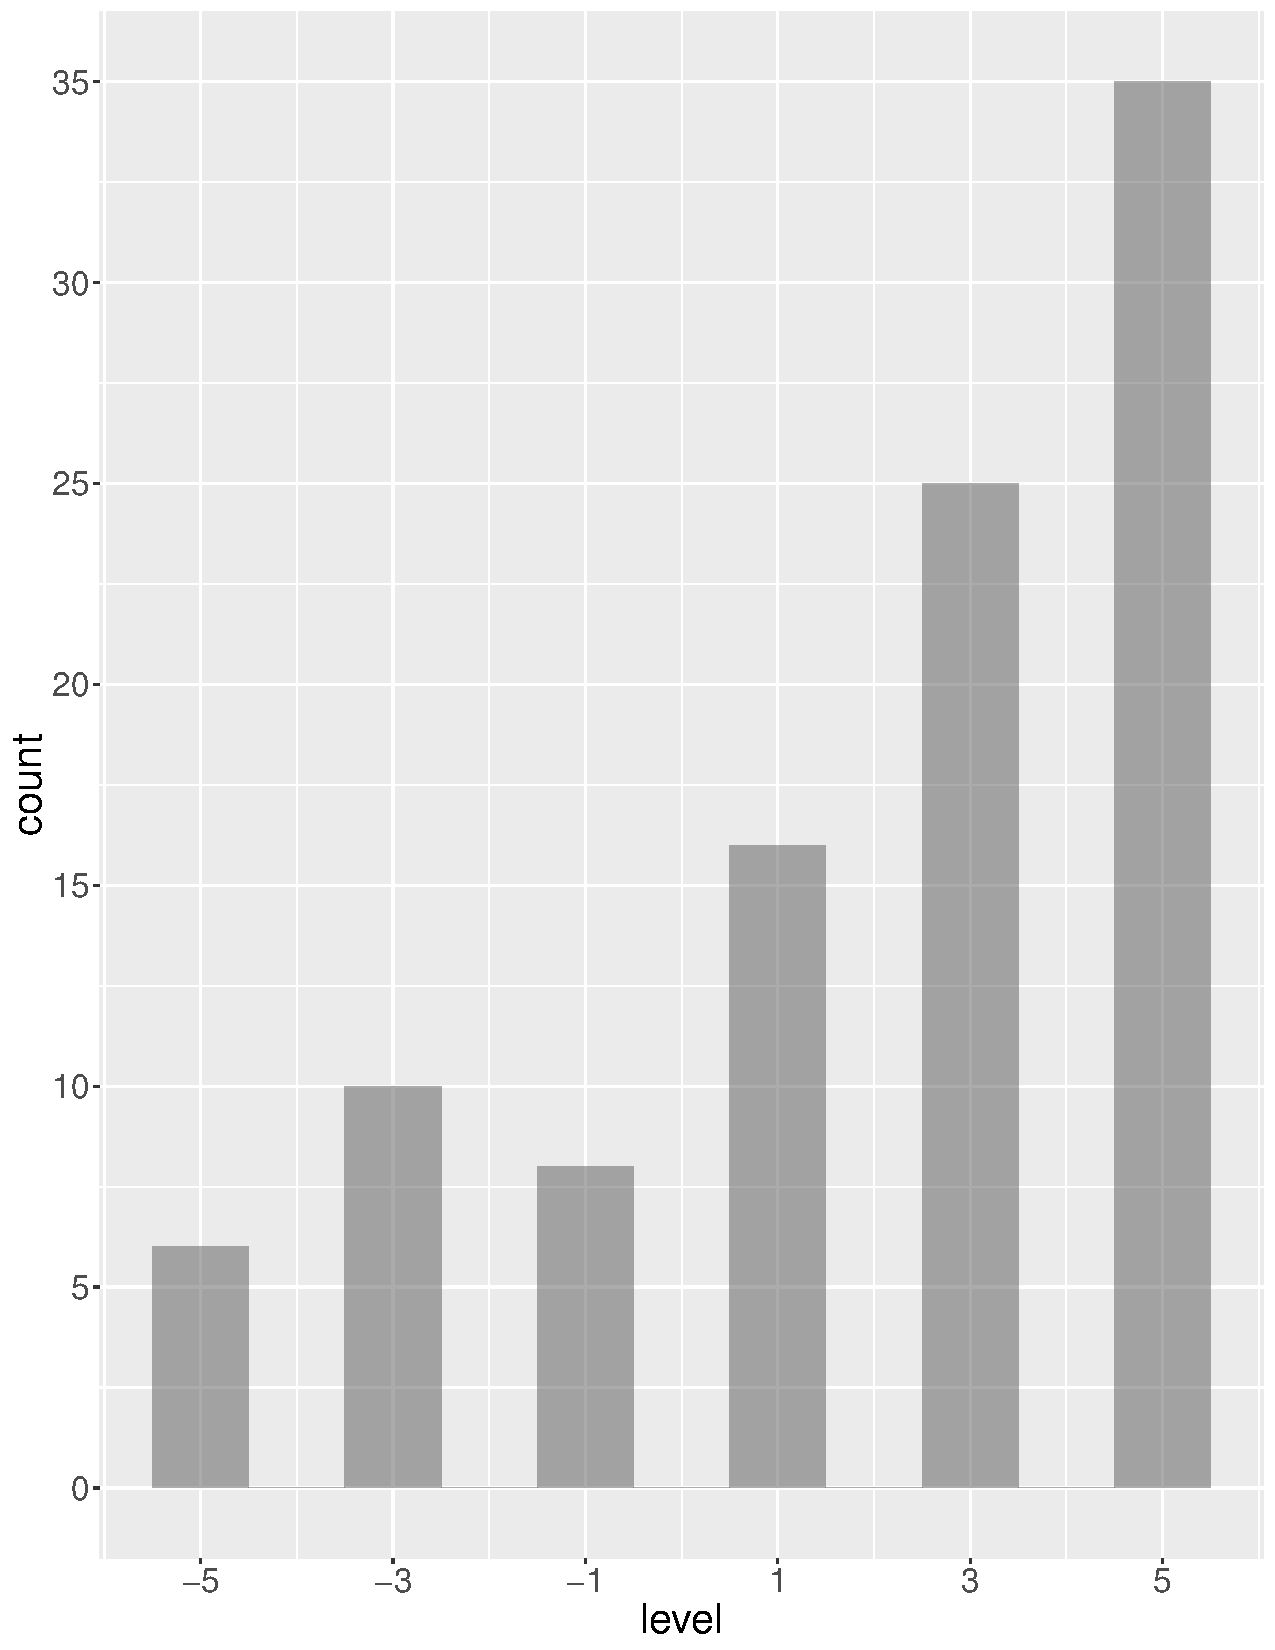
\includegraphics[width=\textwidth]{plots/climate_change/hist_level_nn}
        \caption{Ontology based Approach}
        \label{fig:hist_level_climate_change_nn}
    \end{subfigure}
    ~
    \begin{subfigure}[b]{0.4\textwidth}
        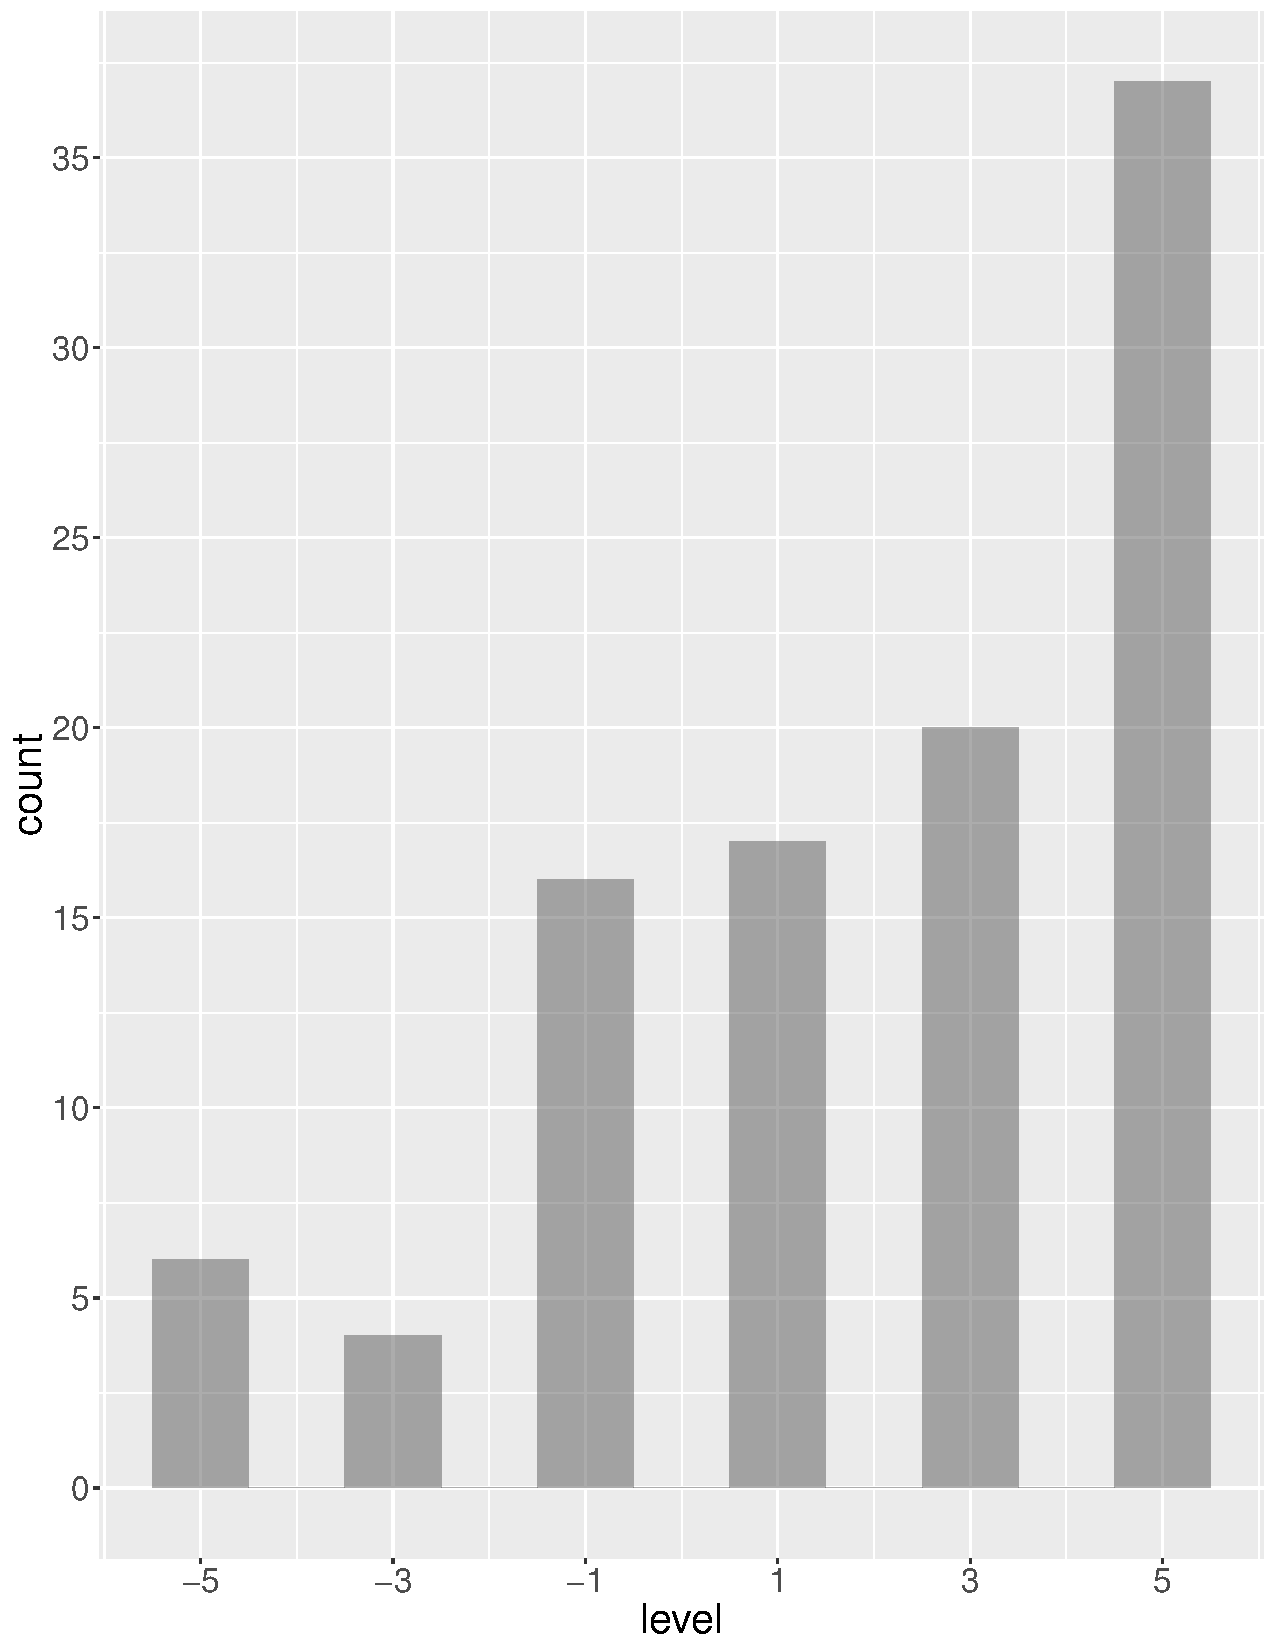
\includegraphics[width=\textwidth]{plots/climate_change/hist_level_ec}
        \caption{Metadata based Approach}
        \label{fig:hist_level_climate_change_ec}
    \end{subfigure}
    ~
    \begin{subfigure}[b]{0.4\textwidth}
        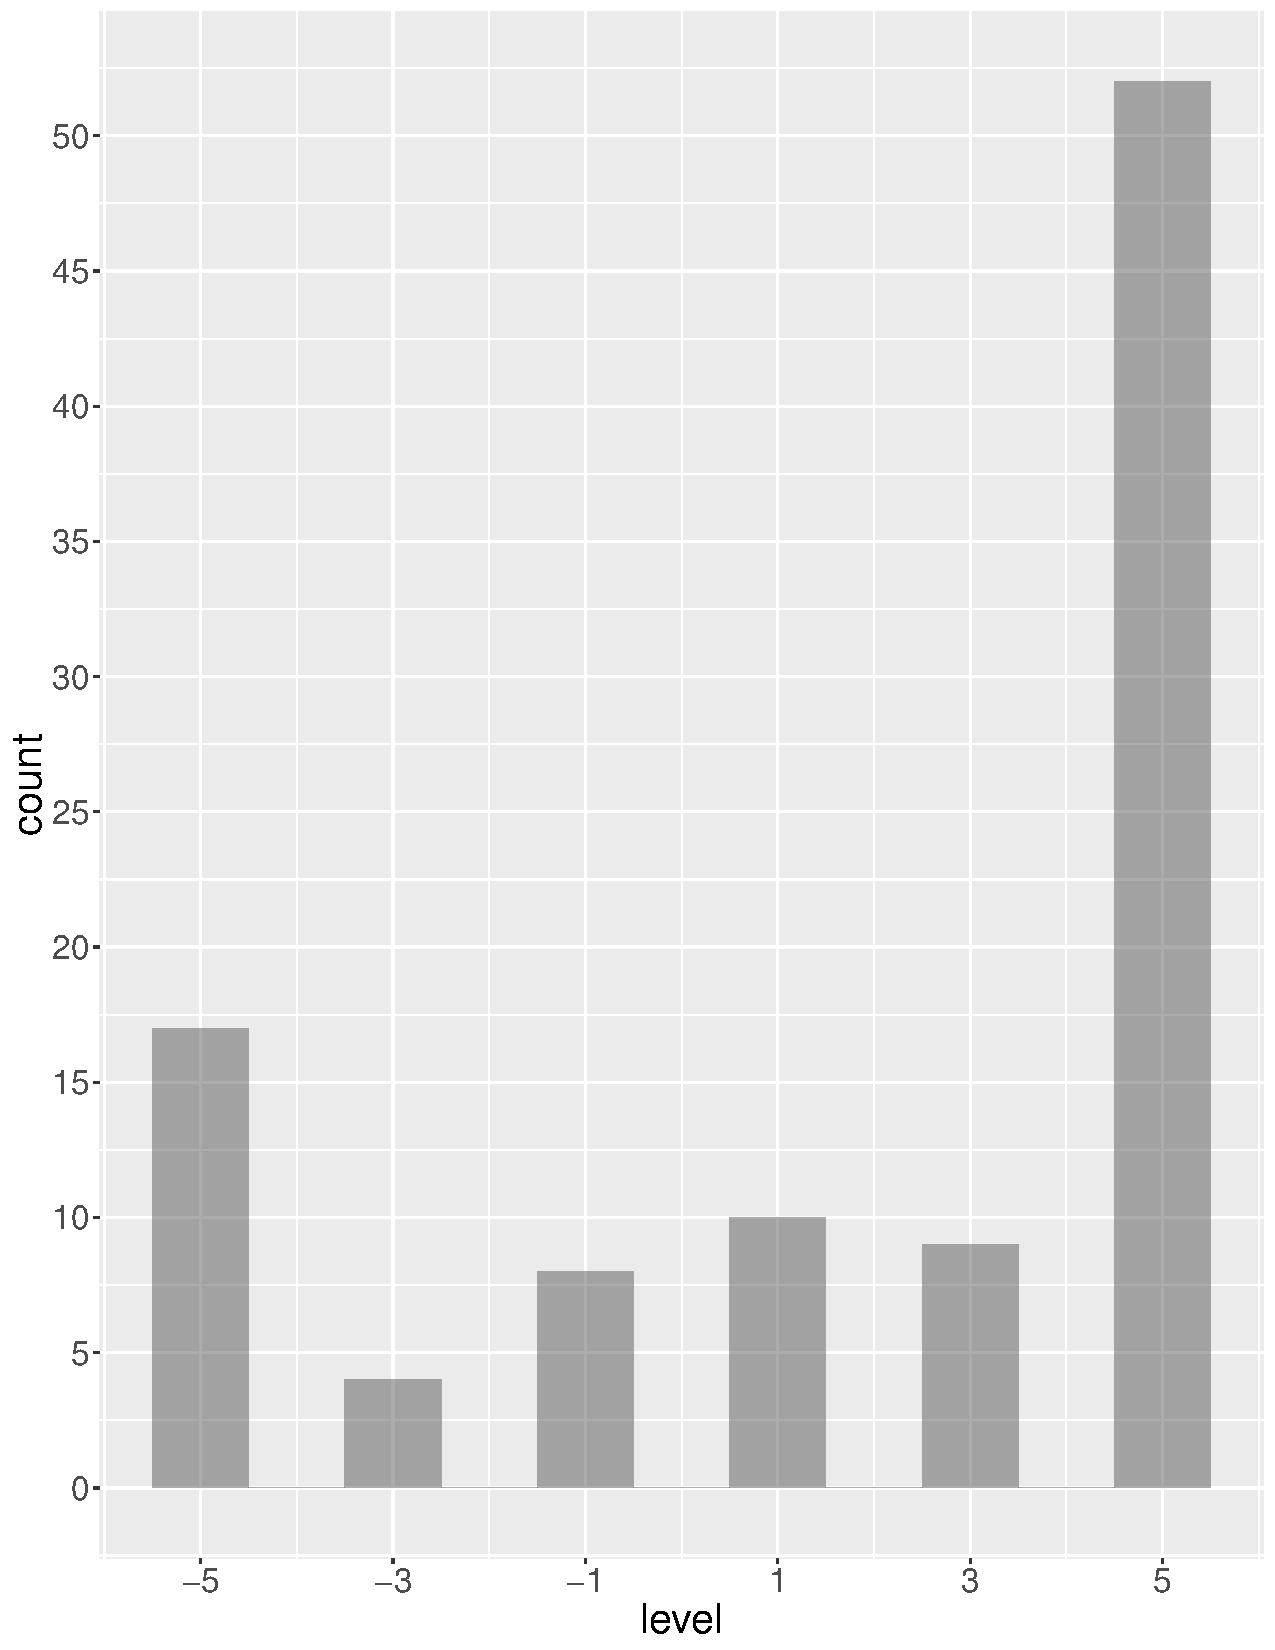
\includegraphics[width=\textwidth]{plots/climate_change/hist_level_es}
        \caption{Dictionary based Approach}
        \label{fig:hist_level_climate_change_es}
    \end{subfigure}
    ~
    \begin{subfigure}[b]{0.4\textwidth}
        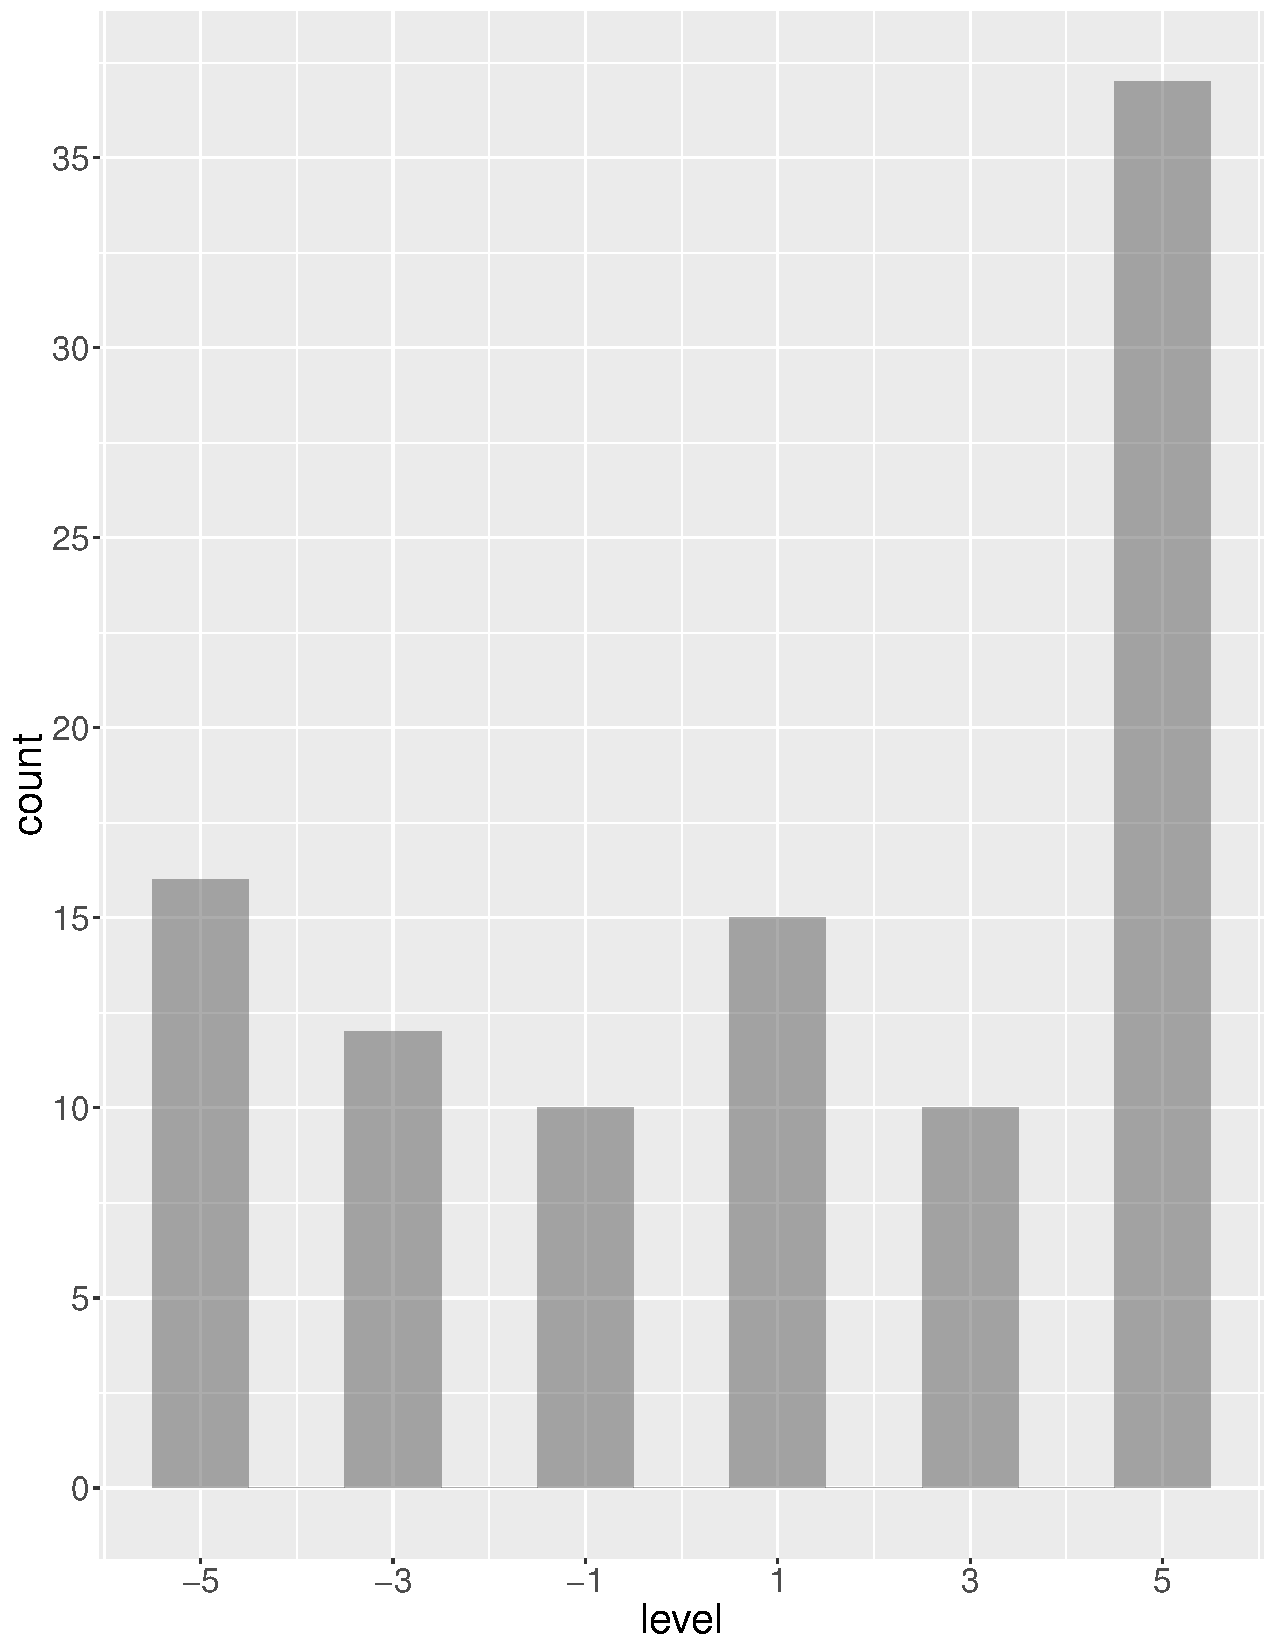
\includegraphics[width=\textwidth]{plots/climate_change/hist_level_none}
        \caption{None}
        \label{fig:hist_level_climate_change_none}
    \end{subfigure}
    \caption{Histogram plots of the correct/incorrect judgements. $\{$\emph{count}=number of judgements, \emph{level}=combined number of correct (positive scale) and incorrect (negative scale) judgements per concept$\}$ }
	\label{fig:hist_level_climate_change_all}
\end{figure}

To manifest our observations from above, bar plots~(illustrated in \hyperref[fig:hist_level_climate_change_all]{Figure~\ref*{fig:hist_level_climate_change_all}}) were created. It combines the agreement ratio and the amount of correct/incorrect judgements. Whereas a negative score indicates that more contributors agreed on incorrect answers or declined relevant concepts, a positive score shows that the majority of crowd worker's responses were correct. Indeed, when comparing the performance on level $-5$ the \emph{Dictionary~based~Approach} is on the same level as if Context was omitted. On the other hand, it shows the highest score of correct answers on level $5$.

Given the plots on the distribution of the correct/incorrect judgements from above, \hyperref[table:level_corr_incorr_climate_change]{Table~\ref*{table:level_corr_incorr_climate_change}} shows the summary statistics of agreement levels for each Context enrichment method. It confirms our observations made so far.
\begingroup
\renewcommand{\arraystretch}{1.5}
\begin{table}
	\begin{tabularx}{\textwidth}{l c*{4}{Y}}
		\toprule
		Method & mean & median & $1^{st}$ quartile & $3^{rd}$ quartile \\
		\midrule
		 Metadata based Approach & 2.04 & 3.00 & -1.00 & 5.00 \\
		 Ontology based Approach & 1.98 & 3.00 & 1.00 & 5.00 \\
		 Dictionary based Approach & 1.92 & 5.00 & -1.00 & 5.00 \\
		 None & 1.04 & 1.00 & -3.00 & 5.00 \\
		\bottomrule
	\end{tabularx}
	\caption{Summary statistics concerning agreement level on the Climate Change Ontology~(ranked by mean value)}
	\label{table:level_corr_incorr_climate_change}
\end{table}
\endgroup
